\newpage
\null
\thispagestyle{empty}
\newpage

\addcontentsline{toc}{chapter}{Ephesians}
% Safely inserts your illustration full-bleed on its own page.
% This completely bypasses the page builder, headers, and geometry bugs!
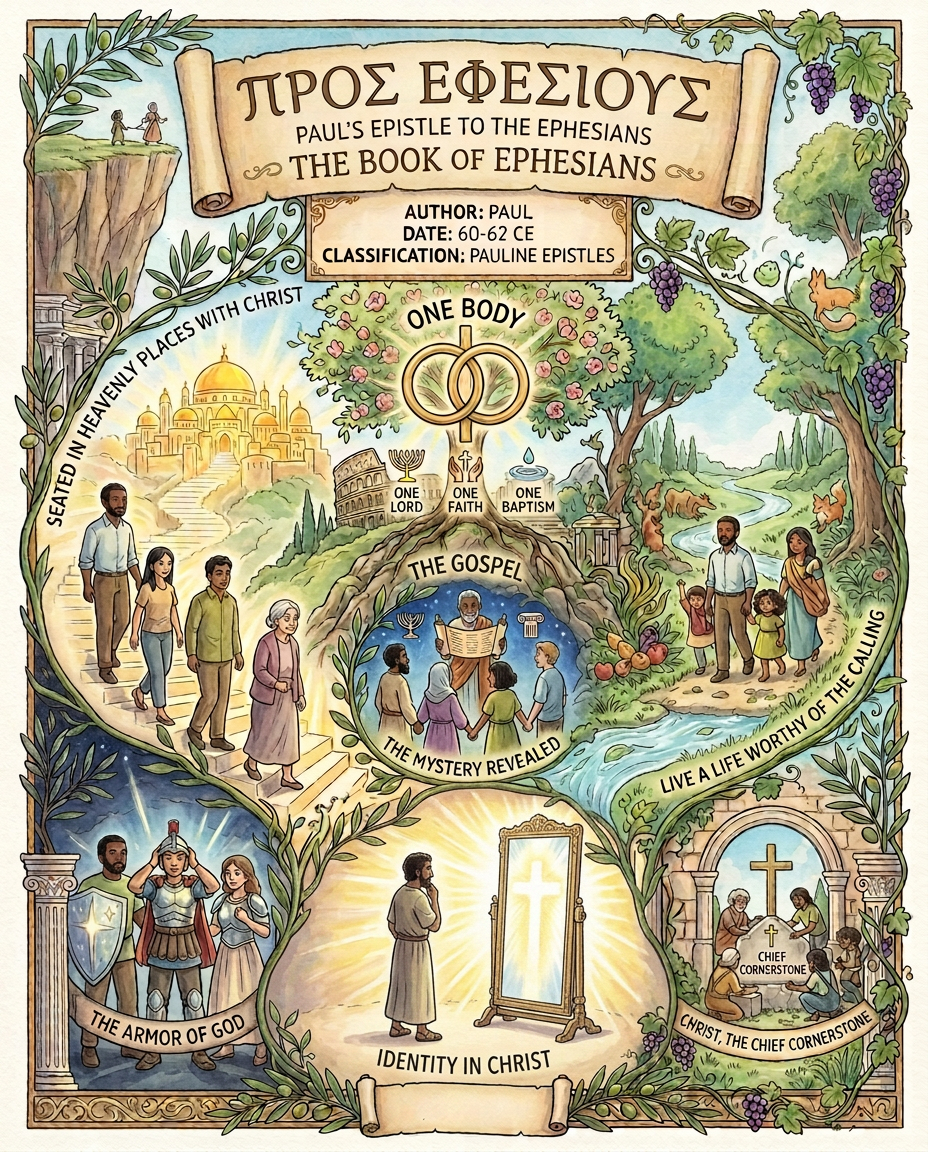
\includepdf[pages=1, fitpaper=false, width=\paperwidth, height=\paperheight, , keepaspectratio=false]{images/divider2/ephesians_2.png}
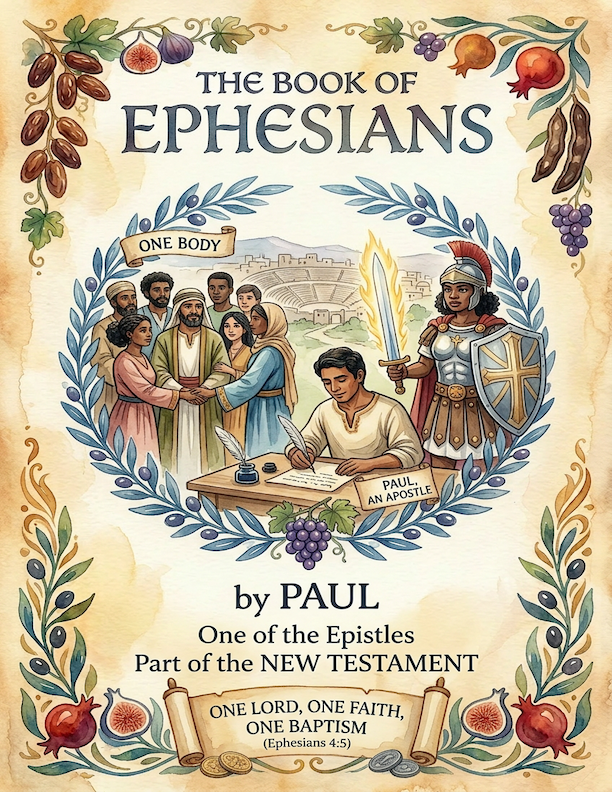
\includepdf[pages=1, fitpaper=false, width=\paperwidth, height=\paperheight, , keepaspectratio=false]{images/divider1/ephesians.png}

\includepdf[pages=1, fitpaper=false, width=\paperwidth, height=\paperheight, , keepaspectratio=false]{images/8.5x11-Dot-Grid.png}

\includepdf[pages=1, fitpaper=false, width=\paperwidth, height=\paperheight, , keepaspectratio=false]{images/8.5x11-Dot-Grid.png}

\mybook{Ephesians}
\vspace{-1.36in}

\mychapter{} \myverse*{}Paul, an emissary of Messiah\footnote{1:1 “Messiah” means “Anointed One”.} Yeshua through the will of God, to the holy ones who
are at Ephesus, and the faithful in Messiah Yeshua:
\myverse{}Grace to you and peace from God our Father and the Lord Yeshua the Messiah.

\myverse{}Blessed be the God and Father of our Lord Yeshua the Messiah, who
has blessed us with every spiritual blessing in the heavenly places in Messiah,
\myverse{}even as he chose us in him before the foundation of the world, that we would
be holy and without defect before him in love,
\myverse{}having predestined us for adoption as children through Yeshua the Messiah to
himself, according to the good pleasure of his desire,
\myverse{}to the praise of the glory of his grace, by which he freely gave us favor in
the Beloved.
\myverse{}In him we have our redemption through his blood, the forgiveness of our trespasses,
according to the riches of his grace
\myverse{}which he made to abound toward us in all wisdom and prudence,
\myverse{}making known to us the mystery of his will, according to his good pleasure which
he purposed in him
\myverse{}to an administration of the fullness of the times, to sum up all things in
Messiah, the things in the heavens and the things on the earth, in him.
\myverse{}We were also assigned an inheritance in him, having been foreordained according
to the purpose of him who does all things after the counsel of his will,
\myverse{}to the end that we should be to the praise of his glory, we who had before
hoped in Messiah.
\myverse{}In him you also, having heard the word of the truth, the Good News of your
salvation—in whom, having also believed, you were sealed with the promised Holy Spirit,
\myverse{}who is a pledge of our inheritance, to the redemption of God’s own possession,
to the praise of his glory.

\myverse{}For this cause I also, having heard of the faith in the Lord
Yeshua which is among you and the love which you have toward all the holy ones,
\myverse{}don’t cease to give thanks for you, making mention of you in my prayers,
\myverse{}that the God of our Lord Yeshua the Messiah, the Father of glory, may give
to you a spirit of wisdom and revelation in the knowledge of him,
\myverse{}having the eyes of your hearts\footnote{1:18 TR reads “understanding” instead of “hearts”} enlightened, that you may know what is
the hope of his calling, and what are the riches of the glory of his inheritance in the holy ones,
\myverse{}and what is the exceeding greatness of his power toward us who believe, according
to that working of the strength of his might
\myverse{}which he worked in Messiah when he raised him from the dead and made him to
sit at his right hand in the heavenly places,
\myverse{}far above all rule, authority, power, dominion, and every name that is named,
not only in this age, but also in that which is to come.
\myverse{}He put all things in subjection under his feet, and gave him to be head over
all things for the assembly,
\myverse{}which is his body, the fullness of him who fills all in all.


% EPHESIANS 2
\mychapter{} \myverse*{}You were made alive when you were dead in transgressions and sins,
\myverse{}in which you once walked according to the course of this world, according to
the prince of the power of the air, the spirit who now works in the children of disobedience.
\myverse{}We also all once lived among them in the lusts of our flesh, doing the desires
of the flesh and of the mind, and were by nature children of wrath, even as the rest.
\myverse{}But God, being rich in mercy, for his great love with which he loved us,
\myverse{}even when we were dead through our trespasses, made us alive together with Messiah—by
grace you have been saved—
\myverse{}and raised us up with him, and made us to sit with him in the heavenly places
in Messiah Yeshua,
\myverse{}that in the ages to come he might show the exceeding riches of his grace in
kindness toward us in Messiah Yeshua;
\myverse{}for by grace you have been saved through faith, and that not of yourselves;
it is the gift of God,
\myverse{}not of works, that no one would boast.
\myverse{}For we are his workmanship, created in Messiah Yeshua for good works, which
God prepared before that we would walk in them.

\myverse{}Therefore remember that once you, the Gentiles in the flesh,
who are called “uncircumcision” by that which is called “circumcision” (in the flesh, made by hands),
\myverse{}that you were at that time separate from Messiah, alienated from the commonwealth
of Israel, and strangers from the covenants of the promise, having no hope and without God in the world.
\myverse{}But now in Messiah Yeshua you who once were far off are made near in the blood
of Messiah.
\myverse{}For he is our peace, who made both one, and broke down the middle wall of
separation,
\myverse{}having abolished in his flesh the hostility, the law of commandments contained
in ordinances, that he might create in himself one new man of the two, making peace,
\myverse{}and might reconcile them both in one body to God through the cross, having
killed the hostility through it.
\myverse{}He came and preached peace to you who were far off and to those who were near.
\myverse{}For through him we both have our access in one Spirit to the Father.
\myverse{}So then you are no longer strangers and foreigners, but you are fellow citizens
with the holy ones and of the household of God,
\myverse{}being built on the foundation of the emissaries and prophets, Messiah Yeshua
himself being the chief cornerstone;
\myverse{}in whom the whole building, fitted together, grows into a holy temple in the
Lord;
\myverse{}in whom you also are built together for a habitation of God in the Spirit.


% EPHESIANS 3
\mychapter{} \myverse*{}For this cause I, Paul, am the prisoner of Messiah Yeshua on behalf
of you Gentiles,
\myverse{}if it is so that you have heard of the administration of that grace of God which
was given me toward you,
\myverse{}how that by revelation the mystery was made known to me, as I wrote before in
few words,
\myverse{}by which, when you read, you can perceive my understanding in the mystery of
Messiah,
\myverse{}which in other generations was not made known to the children of men, as it
has now been revealed to his holy emissaries and prophets in the Spirit,
\myverse{}that the Gentiles are fellow heirs and fellow members of the body, and fellow
partakers of his promise in Messiah Yeshua through the Good News,
\myverse{}of which I was made a servant according to the gift of that grace of God which
was given me according to the working of his power.
\myverse{}To me, the very least of all holy ones, was this grace given, to proclaim to
the Gentiles the unsearchable riches of Messiah,
\myverse{}and to make all men see what is the administration\footnote{3:9 TR reads “fellowship” instead of “administration”} of the mystery which for ages has
been hidden in God, who created all things through Yeshua the Messiah,
\myverse{}to the intent that now through the assembly the manifold wisdom of God might
be made known to the principalities and the powers in the heavenly places,
\myverse{}according to the eternal purpose which he accomplished in Messiah Yeshua our
Lord.
\myverse{}In him we have boldness and access in confidence through our faith in him.
\myverse{}Therefore I ask that you may not lose heart at my troubles for you, which
are your glory.

\myverse{}For this cause, I bow my knees to the Father of our Lord Yeshua the Messiah,
\myverse{}from whom every family in heaven and on earth is named,
\myverse{}that he would grant you, according to the riches of his glory, that you may
be strengthened with power through his Spirit in the inner person,
\myverse{}that Messiah may dwell in your hearts through faith, to the end that you,
being rooted and grounded in love,
\myverse{}may be strengthened to comprehend with all the holy ones what is the width
and length and height and depth,
\myverse{}and to know Messiah’s love which surpasses knowledge, that you may be filled
with all the fullness of God.

\myverse{}Now to him who is able to do exceedingly abundantly above all
that we ask or think, according to the power that works in us,
\myverse{}to him be the glory in the assembly and in Messiah Yeshua to all generations,
forever and ever. Amen.


% EPHESIANS 4
\mychapter{} \myverse*{}I therefore, the prisoner in the Lord, beg you to walk worthily
of the calling with which you were called,
\myverse{}with all lowliness and humility, with patience, bearing with one another in
love,
\myverse{}being eager to keep the unity of the Spirit in the bond of peace.
\myverse{}There is one body and one Spirit, even as you also were called in one hope of
your calling,
\myverse{}one Lord, one faith, one immersion,
\myverse{}one God and Father of all, who is over all and through all and in us all.
\myverse{}But to each one of us, the grace was given according to the measure of the gift
of Messiah.
\myverse{}Therefore he says,

“When he ascended on high,

he led captivity captive,

and gave gifts to people.”\footnote{4:8 Psalms 68:18}

\myverse{}Now this, “He ascended”, what is it but that he also first
descended into the lower parts of the earth?
\myverse{}He who descended is the one who also ascended far above all the heavens, that
he might fill all things.

\myverse{}He gave some to be emissaries; and some, prophets; and some,
evangelists; and some, shepherds\footnote{4:11 or, pastors} and teachers;
\myverse{}for the perfecting of the holy ones, to the work of serving, to the building
up of the body of Messiah,
\myverse{}until we all attain to the unity of the faith and of the knowledge of the
Son of God, to a full grown man, to the measure of the stature of the fullness of Messiah,
\myverse{}that we may no longer be children, tossed back and forth and carried about
with every wind of doctrine, by the trickery of men, in craftiness, after the wiles of error;
\myverse{}but speaking truth in love, we may grow up in all things into him who is the
head, Messiah,
\myverse{}from whom all the body, being fitted and knit together through that which
every joint supplies, according to the working in measure of each individual part, makes the body increase
to the building up of itself in love.

\myverse{}This I say therefore, and testify in the Lord, that you no longer
walk as the rest of the Gentiles also walk, in the futility of their mind,
\myverse{}being darkened in their understanding, alienated from the life of God because
of the ignorance that is in them, because of the hardening of their hearts.
\myverse{}They, having become callous, gave themselves up to lust, to work all uncleanness
with greediness.
\myverse{}But you didn’t learn Messiah that way,
\myverse{}if indeed you heard him and were taught in him, even as truth is in Yeshua:
\myverse{}that you put away, as concerning your former way of life, the old man that
grows corrupt after the lusts of deceit,
\myverse{}and that you be renewed in the spirit of your mind,
\myverse{}and put on the new man, who in the likeness of God has been created in righteousness
and holiness of truth.

\myverse{}Therefore, putting away falsehood, speak truth each one with
his neighbor, for we are members of one another.
\myverse{}“Be angry, and don’t sin.”\footnote{4:26 Psalms 4:4} Don’t let the sun go down on your wrath,
\myverse{}and don’t give place\footnote{4:27 or, opportunity} to the devil.
\myverse{}Let him who stole steal no more; but rather let him labor, producing with
his hands something that is good, that he may have something to give to him who has need.
\myverse{}Let no corrupt speech proceed out of your mouth, but only what is good for
building others up as the need may be, that it may give grace to those who hear.
\myverse{}Don’t grieve the Holy Spirit of God, in whom you were sealed for the day of
redemption.
\myverse{}Let all bitterness, wrath, anger, outcry, and slander be put away from you,
with all malice.
\myverse{}And be kind to one another, tender hearted, forgiving each other, just as
God also in Messiah forgave you.


% EPHESIANS 5
\mychapter{} \myverse*{}Be therefore imitators of God, as beloved children.
\myverse{}Walk in love, even as Messiah also loved us and gave himself up for us, an offering
and a sacrifice to God for a sweet-smelling fragrance.

\myverse{}But sexual immorality, and all uncleanness or covetousness, let
it not even be mentioned among you, as becomes holy ones;
\myverse{}nor filthiness, nor foolish talking, nor jesting, which are not appropriate,
but rather giving of thanks.

\myverse{}Know this for sure, that no sexually immoral person, nor unclean
person, nor covetous man (who is an idolater), has any inheritance in the Kingdom of Messiah and God.

\myverse{}Let no one deceive you with empty words, for because of these things
the wrath of God comes on the children of disobedience.
\myverse{}Therefore don’t be partakers with them.
\myverse{}For you were once darkness, but are now light in the Lord. Walk as children
of light,
\myverse{}for the fruit of the Spirit is in all goodness and righteousness and truth,
\myverse{}proving what is well pleasing to the Lord.
\myverse{}Have no fellowship with the unfruitful deeds of darkness, but rather even
reprove them.
\myverse{}For it is a shame even to speak of the things which are done by them in secret.
\myverse{}But all things, when they are reproved, are revealed by the light, for everything
that reveals is light.
\myverse{}Therefore he says, “Awake, you who sleep, and arise from the dead, and Messiah
will shine on you.”

\myverse{}Therefore watch carefully how you walk, not as unwise, but as
wise,
\myverse{}redeeming the time, because the days are evil.
\myverse{}Therefore, don’t be foolish, but understand what the will of the Lord is.
\myverse{}Don’t be drunken with wine, in which is dissipation, but be filled with the
Spirit,
\myverse{}speaking to one another in psalms, hymns, and spiritual songs; singing and
making melody in your heart to the Lord;
\myverse{}giving thanks always concerning all things in the name of our Lord Yeshua the Messiah
to God, even the Father;
\myverse{}subjecting yourselves to one another in the fear of Messiah.

\myverse{}Wives, be subject to your own husbands, as to the Lord.
\myverse{}For the husband is the head of the wife, as Messiah also is the head of the
assembly, being himself the savior of the body.
\myverse{}But as the assembly is subject to Messiah, so let the wives also be to their
own husbands in everything.

\myverse{}Husbands, love your wives, even as Messiah also loved the assembly
and gave himself up for her,
\myverse{}that he might sanctify her, having cleansed her by the washing of water with
the word,
\myverse{}that he might present the assembly to himself gloriously, not having spot
or wrinkle or any such thing, but that she should be holy and without defect.
\myverse{}Even so husbands also ought to love their own wives as their own bodies. He
who loves his own wife loves himself.
\myverse{}For no man ever hated his own flesh, but nourishes and cherishes it, even
as the Lord also does the assembly,
\myverse{}because we are members of his body, of his flesh and bones.
\myverse{}“For this cause a man will leave his father and mother and will be joined
to his wife. Then the two will become one flesh.”\footnote{5:31 Genesis 2:24}
\myverse{}This mystery is great, but I speak concerning Messiah and the assembly.
\myverse{}Nevertheless each of you must also love his own wife even as himself; and
let the wife see that she respects her husband.


% EPHESISANS 6
\mychapter{} \myverse*{}Children, obey your parents in the Lord, for this is right.
\myverse{}“Honor your father and mother,” which is the first commandment with a promise:
\myverse{}“that it may be well with you, and you may live long on the earth.”\footnote{6:3 Deuteronomy 5:16}

\myverse{}You fathers, don’t provoke your children to wrath, but nurture
them in the discipline and instruction of the Lord.

\myverse{}Servants, be obedient to those who according to the flesh are your
masters, with fear and trembling, in singleness of your heart, as to Messiah,
\myverse{}not in the way of service only when eyes are on you, as men pleasers, but as
servants of Messiah, doing the will of God from the heart,
\myverse{}with good will doing service as to the Lord and not to men,
\myverse{}knowing that whatever good thing each one does, he will receive the same good
again from the Lord, whether he is bound or free.

\myverse{}You masters, do the same things to them, and give up threatening,
knowing that he who is both their Master and yours is in heaven, and there is no partiality with him.

\myverse{}Finally, be strong in the Lord and in the strength of his might.
\myverse{}Put on the whole armor of God, that you may be able to stand against the wiles
of the devil.
\myverse{}For our wrestling is not against flesh and blood, but against the principalities,
against the powers, against the world’s rulers of the darkness of this age, and against the spiritual
forces of wickedness in the heavenly places.
\myverse{}Therefore put on the whole armor of God, that you may be able to withstand
in the evil day, and having done all, to stand.
\myverse{}Stand therefore, having the utility belt of truth buckled around your waist,
and having put on the breastplate of righteousness,
\myverse{}and having fitted your feet with the preparation of the Good News of peace,
\myverse{}above all, taking up the shield of faith, with which you will be able to quench
all the fiery darts of the evil one.
\myverse{}And take the helmet of salvation, and the sword of the Spirit, which is the
word\footnote{6:17 from the Greek “ῥῆμα” (rhema), which means “spoken word”} of God;
\myverse{}with all prayer and requests, praying at all times in the Spirit, and being
watchful to this end in all perseverance and requests for all the holy ones.
\myverse{}Pray for me, that utterance may be given to me in opening my mouth, to make
known with boldness the mystery of the Good News,
\myverse{}for which I am an ambassador in chains; that in it I may speak boldly, as
I ought to speak.

\myverse{}But that you also may know my affairs, how I am doing, Tychicus,
the beloved brother and faithful servant in the Lord, will make known to you all things.
\myverse{}I have sent him to you for this very purpose, that you may know our state
and that he may comfort your hearts.

\myverse{}Peace be to the brothers, and love with faith, from God the Father
and the Lord Yeshua the Messiah.
\myverse{}Grace be with all those who love our Lord Yeshua the Messiah with incorruptible
love. Amen.


